\newpage
\section{Präzession}
Zuerst soll das Produkt der Winkelgeschwindigkeiten \(\omega_3 \cdot \omega_\text{p}\) gegen \(\omega_3\) aufgetragen werden.
Es gilt:
\begin{align}
    \omega_3 &= 2\pi f_3 \\
    \omega_3 \cdot \omega_\text{p} &= 4 \pi^2 \, \frac{f_3}{T_\text{p}}
\end{align}
Wobei \(f_3\) die Rotationsfrequenz ist, die im Messprotokoll fälschlicherweise mit \(\omega_3 \) benannt wurde, und \(T_\text{p}\) die Zeit für eine Präzessionsumdrehung ist.
Es ergeben sich folgende Werte:\\
Messreihe 2:\\
\begin{table}[h]
    \centering
    \begin{tabular}{c|c|c|c|c}
            \(f_3\) in Hz & \(T_p\) in s & \(\omega_3\) in 1/s & \(\omega_3 \cdot \omega_\text{p}\) in 1/s\textsuperscript{2} &   \(s_{\omega_3 \cdot \omega_\text{p}}\) in 1/s\textsuperscript{2} \\
            \hline
            16,72 &  57,53 &  105,054858 &  11,473651 &  0,357309 \\
            14,61 &  49,58 &   91,797337 &  11,633313 &  0,415054 \\
            12,89 &  43,78 &   80,990259 &  11,623499 &  0,470009 \\
            11,52 &  39,62 &   72,382295 &  11,478833 &  0,518846 \\
            10,41 &  36,00 &   65,407959 &  11,415842 &  0,570775 \\
             9,50 &  32,98 &   59,690260 &  11,371891 &  0,622857 \\
             8,66 &  30,96 &   54,412385 &  11,042736 &  0,662044 \\
             8,09 &  28,12 &   50,830969 &  11,357767 &  0,730436 \\
             7,60 &  25,13 &   47,752208 &  11,939354 &  0,820619 \\
             7,02 &  24,48 &   44,107961 &  11,321017 &  0,838840 \\
        \end{tabular}
        \caption{Wertetabelle: Präzession - Messreihe 2}
\end{table}

Messreihe 3:
\begin{table}[h]
    \centering
    \begin{tabular}{c|c|c|c|c}
        \(f_3\) in Hz & \(T_\text{p}\) in s & \(\omega_3\) in 1/s  & \(\omega_3 \cdot \omega_\text{p}\) in 1/s\textsuperscript{2} & \(s_{\omega_3 \cdot \omega_\text{p}}\) in 1/s\textsuperscript{2} \\
        \hline
        16,86 &  57,19 &  105,934504 &  11,638505 &  0,359838 \\
        14,52 &  49,15 &   91,231851 &  11,662800 &  0,418770 \\
        12,77 &  44,19 &   80,236276 &  11,408450 &  0,464967 \\
        11,43 &  37,96 &   71,816808 &  11,887205 &  0,543062 \\
        10,23 &  35,70 &   64,276986 &  11,312723 &  0,575172 \\
        9,36 &  32,00 &   58,810614 &  11,547437 &  0,642696 \\
        8,49 &  29,95 &   53,344243 &  11,191044 &  0,685041 \\
        7,90 &  28,03 &   49,637164 &  11,126632 &  0,731652 \\
        7,40 &  25,71 &   46,495571 &  11,362905 &  0,798933 \\
        6,94 &  24,02 &   43,605306 &  11,406337 &  0,855395 \\
        \end{tabular}
        \caption{Wertetabelle: Präzession - Messreihe 3}
\end{table}\\
Für die Fehler gilt:
\begin{align}
    s_{\text{f}_3} &= 0,5 \, \text{Hz} \\
    s_{\text{T}_p} &= 0,5 \, \text{s}  \\
    s_{\omega_3 \cdot \omega_\text{p}} &= 4\pi^2 \sqrt{(\frac{s_{\text{f}_3}}{T_\text{p}})^2 + (\frac{f_3}{T_\text{p}^2} s_{\text{T}_p})^2}
\end{align}
\newpage
Trägt man nun \(\omega_3 \cdot \omega_\text{p}\) gegen \(\omega_3\) auf, so ergibt sich folgendes Grafik:
\begin{figure}[h]
    \centering
    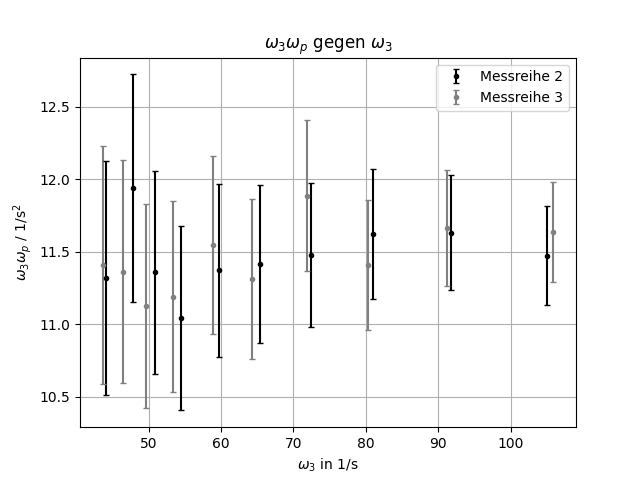
\includegraphics[width=0.6\textwidth]{6.3/Figure_1.png}
    \caption{Präzession}%\(\omega_3 \cdot \omega_\text{p}\) gegen \(\omega_3\) aufgetragen}
\end{figure}

Da es sich bei \(\omega_3 \cdot \omega_\text{p}\) um eine Konstante handelt bedinen wir uns der Statistik um einen genaueren Wert zu ermitteln.
\begin{figure}[h]
    \centering
    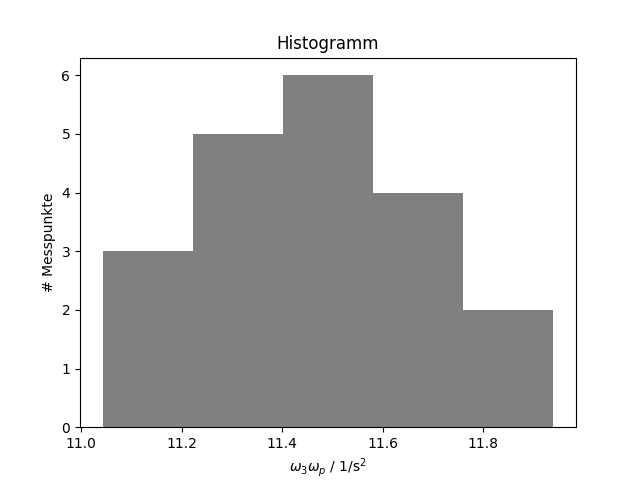
\includegraphics[width=0.6\textwidth]{6.3/Figure_2.png}
    \caption{Histogramm der errechneten Werte}% \(\omega_3 \cdot \omega_\text{p}\)}
\end{figure}\\

Somit ergibt sich als Mittelwert und die Standardabweichungdes Mittelwerts: 
\begin{align}
    \omega_3 \cdot \omega_\text{p} = (11,46 \pm 0,05) \, \frac{1}{\text{s}^2}
\end{align}
Für diese Berechnung wurden folgende Formeln verwendet:
\begin{align}
    \omega_3 \cdot \omega_\text{p} &= \frac{1}{n}\sum_{i=1}^n (\omega_3 \cdot \omega_\text{p})_\text{(i)}\\
    s_{\omega_3 \cdot \omega_\text{p}} &= \frac{1}{\sqrt{n}} \sqrt{\frac{1}{n-1}\sum_{i=1}^n((\omega_3 \cdot \omega_\text{p})_\text{(i)} - \overline{(\omega_3 \cdot \omega_\text{p})})^2}
\end{align}
Wobei \(n\) die Anzahl der Messwerte ist.



Mit hilfe der Gleichung (12) aus der Versuchsanleitung lässt sich folgende Formel für das Trägheitsmoment herleiten:
\begin{align}
    J_3 = \frac{mgl}{\omega_3 \cdot \omega_\text{p}}\\
    s_{J_3} = 4\pi^2 \sqrt{(\frac{s_{f_3}}{T_\text{p}})^2 + (\frac{f_3}{T_\text{p}^2} s_{T_\text{p}})^2}
\end{align}
Der Fehler der Frequenz wurde, aufgrund der Messmethode, mit \(s_{f_3} = 0,5\) Hz veranschlagt.
Durch einsetzen der Werte:
\begin{align}
    m = (48,3 \pm 0,02)\, \text{g}\\
    l = (96,2 \pm 0,1)\, \text{mm}
\end{align}
folgt
\begin{align}
    J_3 = (3,98 \pm 0,03) \cdot 10^{-3} \, \text{kg m}^2
\end{align}

Aus der vorherigen Aufgabe wissen wir:
\begin{align}
    J_1 = \frac{J_3}{\frac{\omega_\text{n}}{\omega_3}+1}
\end{align}
Für den Fehler gilt also:
\begin{align}
    s_{J_1} = \frac{1}{\frac{\omega_\text{n}}{\omega_3}+1} \sqrt{s_{J_3}^2 + (\frac{J_3}{\frac{\omega_n}{\omega_3}+1} s_{\frac{\omega_n}{\omega_3}})^2}
\end{align}
Somit ergibt sich:
\begin{align}
    J_1 = (4,05 \pm 0,03)\cdot 10^{-3} \, \text{kg m}^2
\end{align}

Wie zu erwarten war gilt \(J_3 < J_1\) und sie unterscheiden sich nur geringfügig, da der Kreisel näherungsweise eine Kugel ist.

Um nun besser einschätzen zu können ob die Werte plausibel sind vergleichen wir sie mit denen einer ähnlich dimensionierten Stahlkugel.

Für das Trägheitsmoment einer Kugel gilt:
\begin{align}
    J = \frac{8}{15}\pi\varrho r^5
\end{align}
Für den Radius setzen wir \(r = 0,05\)m an und für die Dichte von Stahl gilt \(\varrho \approx 7700\, \frac{\text{kg}}{\text{m}^3}\).

Mit diesen Werten ergibt sich ein Trägheitsmoment von \(J \approx 4,03 \cdot 10^{-3}\) kg m\textsuperscript{2}, welcher sehr gut zu den von uns ermittelten passt.